\documentclass{article}
\usepackage[utf8]{inputenc}

\title{MATH3160 — Portfolio 4.3}
\author{Mike Medved}
\date{October 25th, 2022}

\usepackage{color}
\usepackage{amsthm}
\usepackage{amssymb} 
\usepackage{amsmath}
\usepackage[margin=1in]{geometry} 
\usepackage{listings}
\usepackage[dvipsnames]{xcolor}
\usepackage{tikz}

\newtheorem*{thm}{Theorem}

\begin{document}

\maketitle

\section{Deliverables}

\subsection{Probability Density Function (pdf)}

The density of a continuous random variable $X$ is by definition the probability that $X$ takes a value in an open or closed interval $[a,b]$. The probability density function (pdf) itself is on the domain of $f \colon \mathbb{R} \to [0, \infty]$, and can be simply defined as the following integral:

$$
P(X \in I) = \int_{I} f(x) \, dx
$$

$\hfill \break$
An example of using it to find if $X$ takes values in a given interval is shown below.

$\hfill \break$
This solution refers to a random variable whose density is given as the following:

$$
\begin{cases}
\frac{1}{10}e^{-\frac{1}{10}x} & x \geq 0 \\
0 & x < 0    
\end{cases}
$$

$\hfill \break$

\begin{center}
    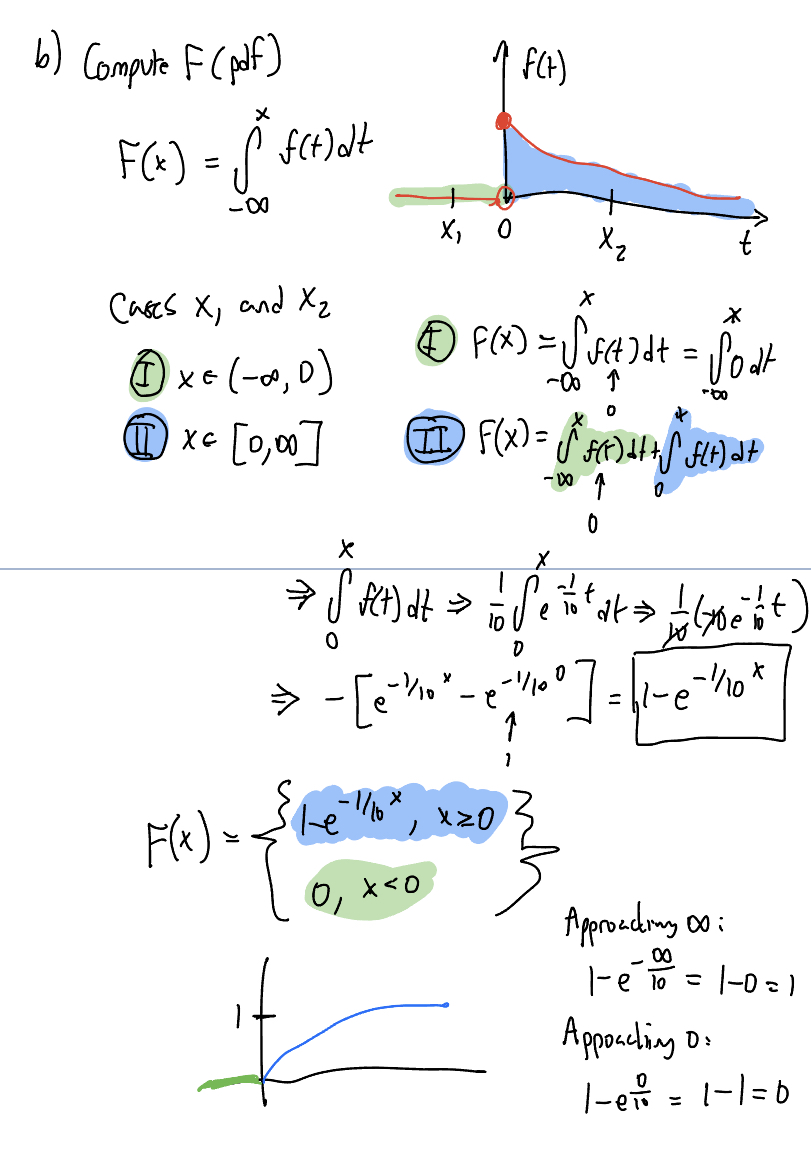
\includegraphics[height=4in]{pdf.jpeg}
\end{center}

\subsection{Cumulative Distribution Function (cdf)}

The distribution of a continuous random variable $X$ is by definition the probability that $X$ takes a value less than or equal to a given cutoff $x$. The cumulative distribution function (cdf) itself is on the domain of $F \colon \mathbb{R} \to [0, 1]$, and can be simply defined as the following integral:

$$
F(X) = P(X \leq x) = P(X \in (-\infty, x]) = \int_{-\infty}^{x} f(t) \, dt
$$

$\hfill \break$
The following are the four properties of the continuous distribution function:

\begin{enumerate}
    \item $\displaystyle\lim_{x \to -\infty} f(x) = 0$
    \item $\displaystyle\lim_{x \to +\infty} f(x) = 1$
    \item F is increasing
    \item F is continuous
\end{enumerate}

\subsection{Example of finding distribution using density}

Using the example from Section 1.1, we can see that the density function is given as:

$$
\begin{cases}
\frac{1}{10}e^{-\frac{1}{10}x} & x \geq 0 \\
0 & x < 0
\end{cases}
$$

$\hfill \break$
From this, we computed the the pdf to be $1-e^{\frac{1}{10}x}$ for an arbitrary input $x$. Given this, we can differentiate the pdf to find the cdf:

\begin{align*}
F(X) &= 1-e^{\frac{1}{10}x} \\
&= -(-\frac{1}{10})e^{-\frac{1}{10}} \\
&= \frac{1}{10}e^{-\frac{1}{10}x} \\
\end{align*}

\subsection{Continuous formulas for E[X], Var[X], and mgf(X)}

The formula for the expectation, $E[X]$, of a continuous random variable $X$ is given as:

$$
E[X] = \int_{\mathbb{R}} x \cdot f(x) \, dx
$$

$\hfill \break$
The formula for the variance of a continuous random variable $X$ is unchanged from the discrete case:

$$
\textit{Var(X)} = E[(X-E[X])^2]
$$

$\hfill \break$
The formula for the moment generating function of a continuous random variable $X$ is given on the domain of $M_X \colon \mathbb{R} \to [-\infty, \infty]$, and has the following formula:

$$
M_X(t) = E\left[e^{tX}\right]
$$

\subsection{Example of using density to find E[X], Var(X), and mgf(X)}

Below is a problem that solves for the expectation, variance, and moment generating function of a continuous random variable $X$.

\begin{center}
    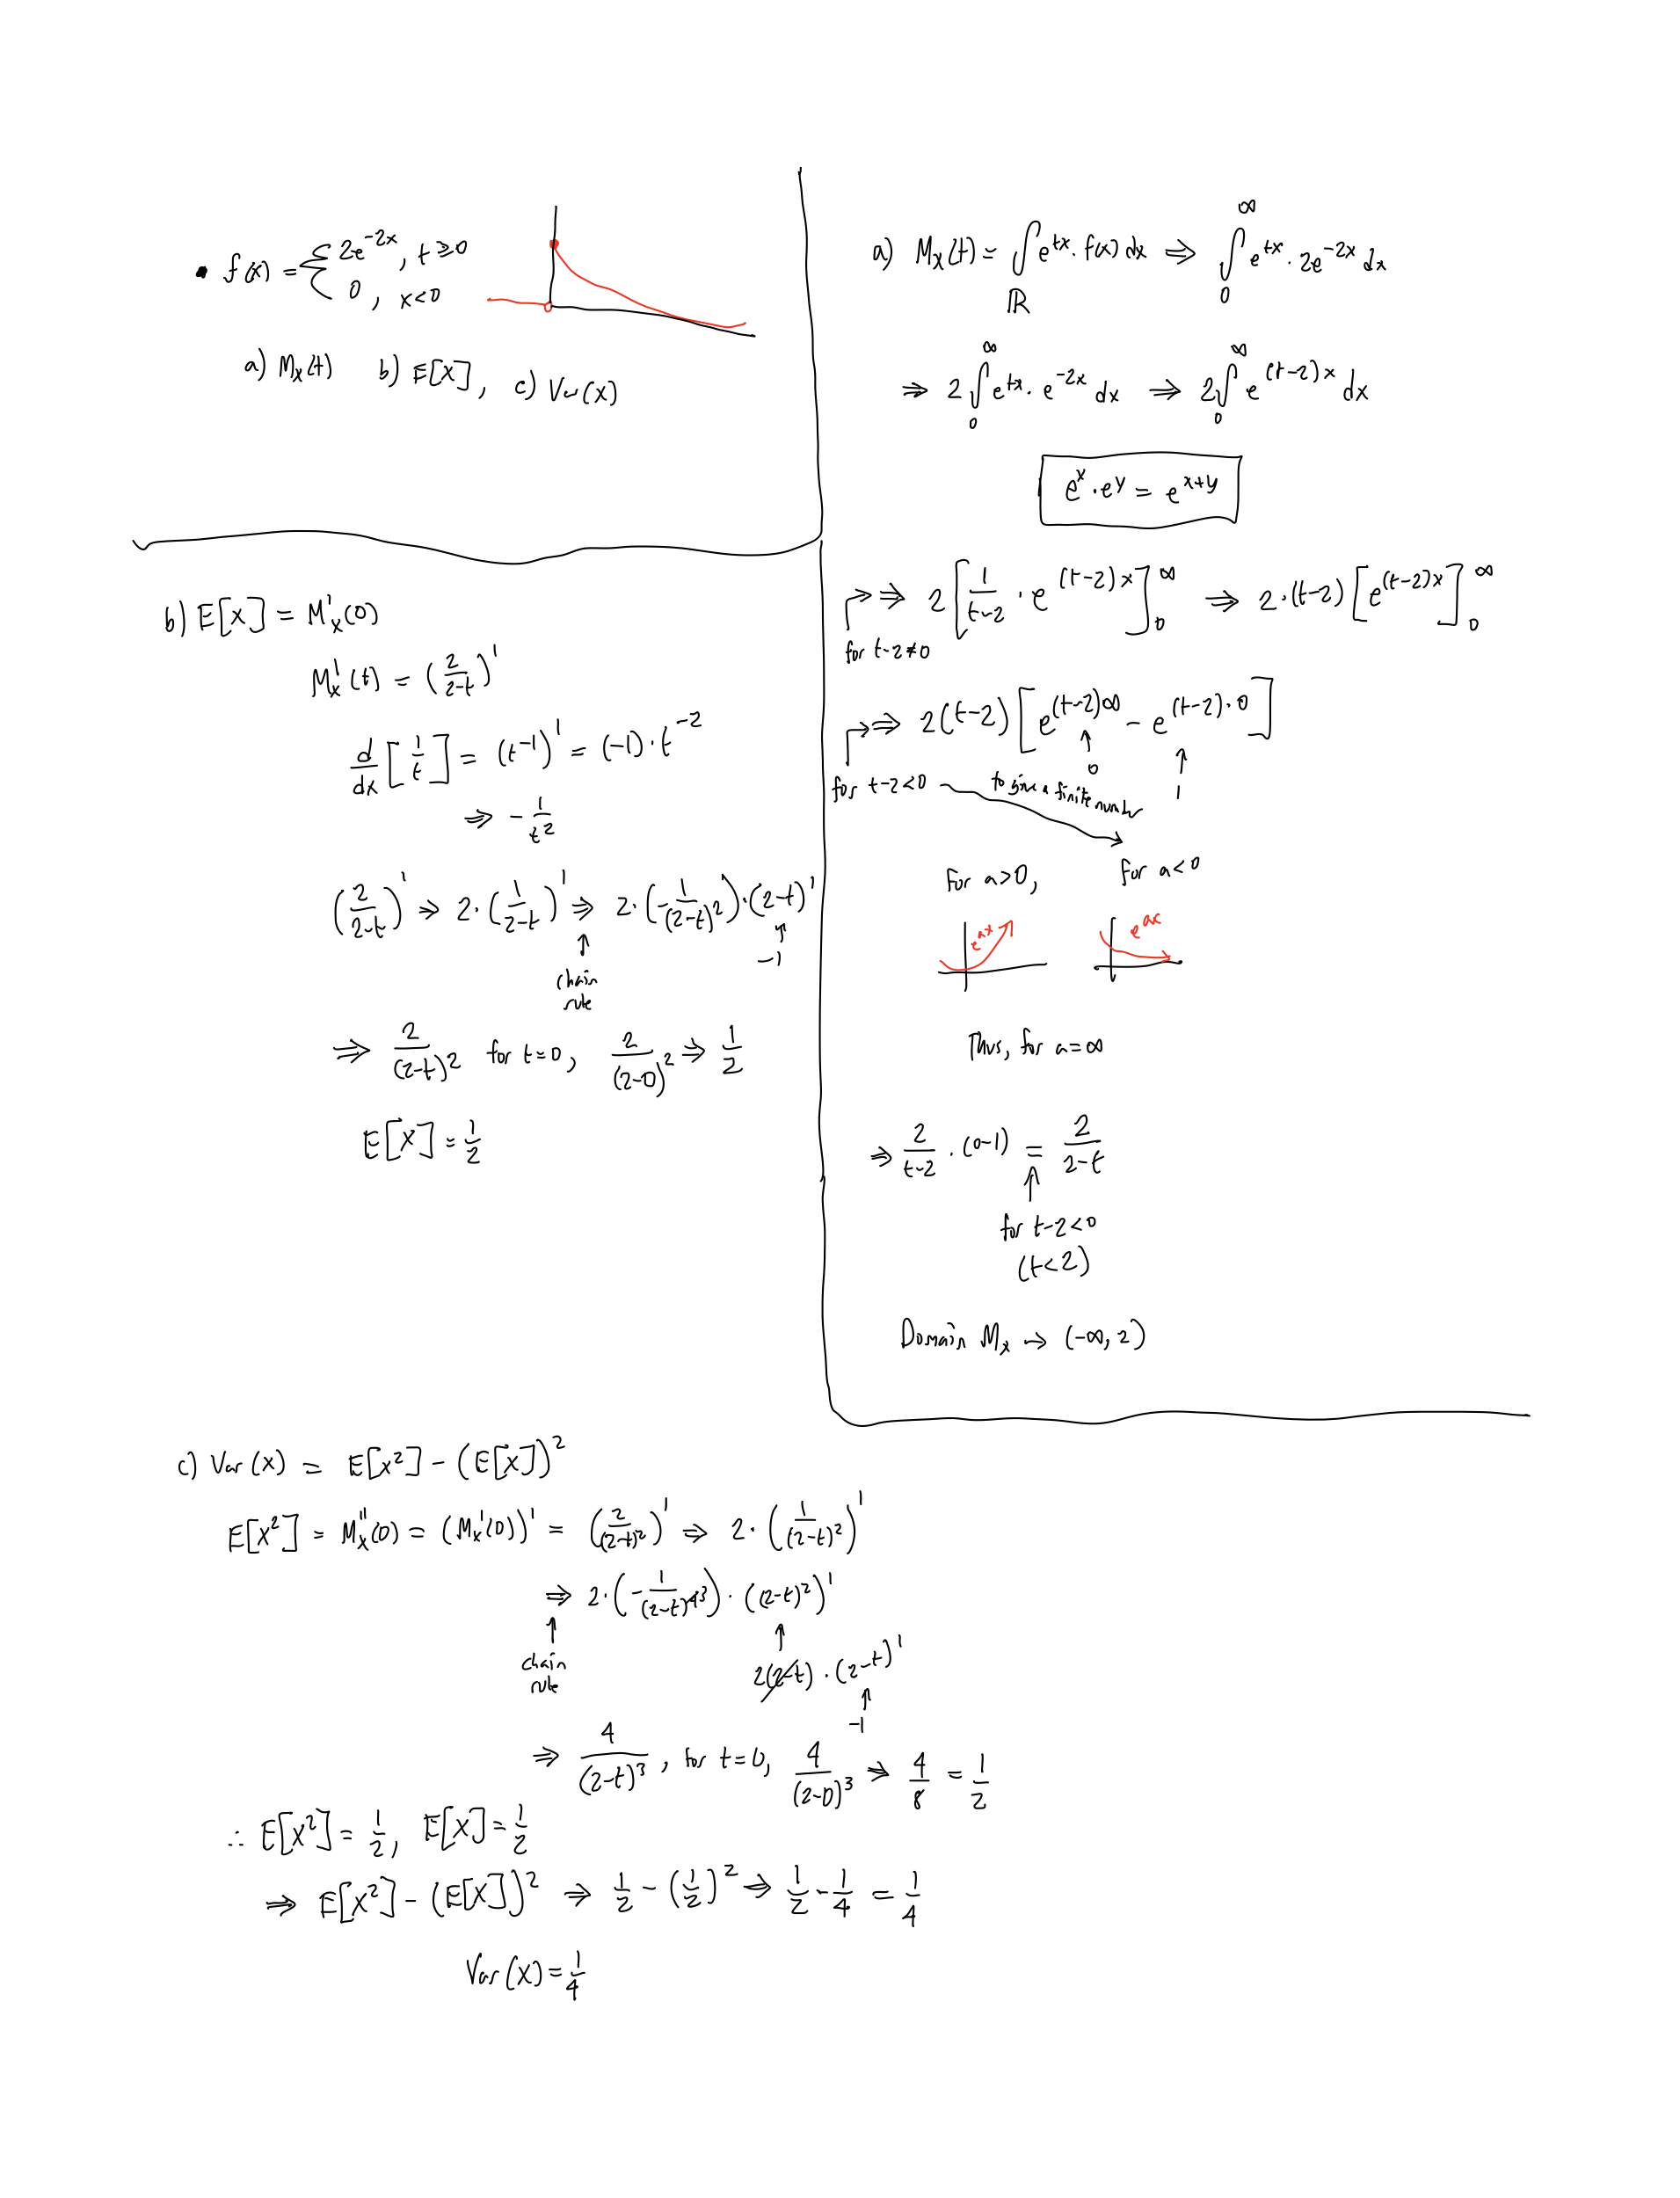
\includegraphics[height=8in]{e-var-mgf.png}
\end{center}

\end{document}